\textbf{Bài 1.1:}
\begin{enumerate}[label=(\alph*)]
    \item Hàm số xác định nếu \(2x-1\neq 0\), hay \(x\neq \frac{1}{2}\). Vì vậy \(X=(-\infty, 1/2)\cup (1/2,\infty)\).
    \item Hàm này xác định nếu \(x-1\neq 0\) và \(1+x>0\), hay \(x\neq 1\) và \(x>-1\). Vì vậy \(X=(-1,1)\cup (1,\infty)\).
    \item Số hạng thứ nhất nhận các giá trị thực khi \(x\leq\frac{1}{2}\). Số hạng thứ hai nhận các giá trị thực khi \(-1\leq\frac{3x-1}{2}\leq 1.\) Giải ra ta được \(x\leq 1, x\geq -\frac{1}{3}\). Do đó miền xác định là đoạn \([-1/3,1/2]\).
    \item Hàm số xác định với \(x\neq 0\). Nên \(X=(-\infty, 0)\cup(0,\infty)\).
    \item Điều kiện để hàm số xác định là \(3x+1\geq 0\) và \(x+1\geq 0\). Vậy \(X=[-1/3,\infty)\).
\end{enumerate}
\vspace{5pt}

\textbf{Bài 1.2:}
\begin{enumerate}[label=(\alph*)]
    \item Biến đổi, ta được \(f(x)=(x-3)^2 -4 \geq -4\). Do đó tập hợp giá trị của hàm là khoảng \(Y=[-4, \infty)\).
    \item Vì \(-1\leq \sin x\leq 1\), nên \(-3\leq\sin x\leq 3\). Do đó \(-1\leq f(x)\leq 5\) và \(Y=[-1, 5]\).
    \item Ta xem xét hai trường hợp : \(x<0 \text{ và } x>0\). \newline Nếu \(x<0\), \(y+\lvert y\rvert =1\). Giá trị của \(y\) không thể nhỏ hơn \(0\) vì điều này tương đương với \(y+\lvert y\rvert =0\). Do đó \(y=\frac{1}{2}\) trong trường hợp này.\newline Nếu \(x>0\), \(y\) chắc chắn lớn hơn \(0\) và do đó ta thu được hàm \(y=x+\frac{1}{2}\).\newline Dễ thấy, miền giá trị \(Y=[1/2,\infty)\).
    \item Miền giá trị của hàm là \(Y=[0,4]\).
\end{enumerate}
\vspace{5pt}

\textbf{Bài 1.3:}

Xét đường tròn tâm \(O\) có đường kính \(AC\) với độ dài bằng \(1\) và tứ giác \(ABCD\) nội tiếp đường tròn như hình bên.\raisebox{-0.2em}{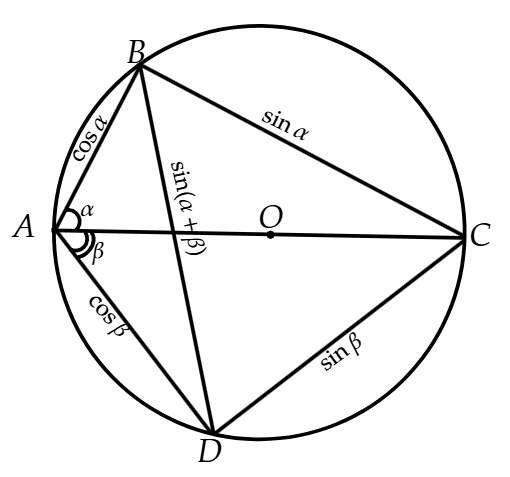
\includegraphics[height=8 cm]{Tuan1/ảnh/unitcircle.png}}\newline
Vì \(\lvert AC\rvert =1\) nên tất cả độ dài trong biểu đồ được kết nối với sine hoặc cosine, và chú ý rằng hai góc ở đỉnh \(B\) và \(D\) là các góc vuông.\newline
Lúc này, theo định lý hàm sine trong tam giác, độ dài đoạn \(BD\) chính là \(\sin(\alpha+\beta)\). Định lý Ptoleme lại cho biết rằng \[\lvert AC\rvert \cdot\lvert BD\rvert =\lvert AB\rvert\dot\lvert CD\rvert +\lvert BC\rvert\dot\lvert AD\rvert.\]
và biểu thức này trở thành, sau khi ta thay các giá trị sine/cosine tương ứng:\[\sin(\alpha+\beta)=\sin\alpha\cos\beta +\sin\beta\cos\alpha.~(Q.E.D)\]
Sử dụng định lý Pythagoras, ta chứng minh được đẳng thức còn lại.

\vspace{5pt}
\textbf{Bài 1.4:}
